\documentclass[t,aspectratio=169]{beamer}
%\usetheme{Berkeley}
\usepackage{graphicx}
\usepackage{amsmath}
\usepackage[american]{circuitikz}

\title{Clase 14}
\subtitle{El transistor BJT en CD}
\author{Dr.-Ing. Juan José Montero Rodríguez}
\subject{Elementos Activos}
\institute{Escuela de Ingeniería Electrónica}
\date{Semestre II-2023}

\begin{document}

\begin{frame}{}
\maketitle
\end{frame}


\section{Fundamentos}
\begin{frame}{El modelo CD del transistor BJT}
\begin{itemize}
    \item Se coloca un diodo entre la base y el emisor.
    \item Se coloca una fuente de corriente dependiente entre el colector y el emisor.
\end{itemize}

\begin{figure}
    \centering
    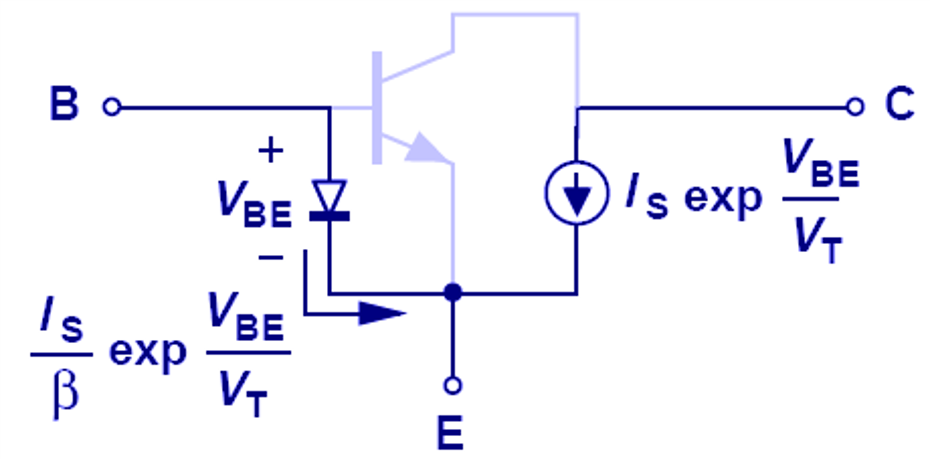
\includegraphics[width=0.7\textwidth]{figures/modelo_cd_bjt.png}
\end{figure}

\end{frame}


\begin{frame}{El modelo CD del transistor BJT}

\begin{columns}
\begin{column}{0.5\textwidth}
\centering
\textbf{Relaciones de corriente}
\[ I_C = \beta I_B \]
\[ I_E = (\beta + 1) I_B \]
\[ I_E = I_B + I_C \]

\textbf{Ganancias de corriente}
\[ \beta = \dfrac{I_C}{I_B} \]
\[ \alpha = \dfrac{I_C}{I_E} \]

\end{column}
\begin{column}{0.5\textwidth}
\centering
\textbf{Modelo de tensión constante}
\[ V_{BE} \approx 0.7\ V \]

\textbf{Modelo exponencial}
\[ I_C = I_S \cdot e^{V_{BE}/V_t} \]
\[ V_{BE} = V_t \ln (I_C / I_S) \]

\flushleft
\begin{itemize}
    \item Las ecuaciones son válidas únicamente en activa directa.
\end{itemize}

\end{column}
\end{columns}

\end{frame}


\begin{frame}{Solución de circuitos por recta de carga}

Se busca la intersección de un sistema de dos ecuaciones: la ecuación del circuito, y la ecuación del transistor.

\begin{figure}
    \centering
    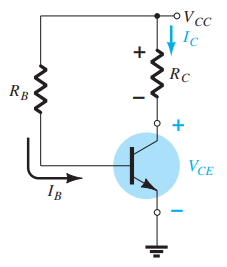
\includegraphics[width=4cm]{figures/recta_de_carga_bjt_2.png}\hspace{1cm}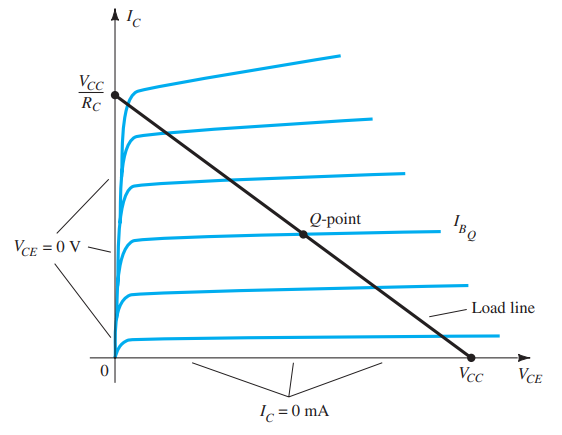
\includegraphics[width=7cm]{figures/recta_de_carga_bjt.png}
\end{figure}

\end{frame}



\section{Ejemplo 1}
\begin{frame}{Ejemplo 1: Cálculo del punto de operación NPN}

\begin{columns}
\begin{column}{0.6\textwidth}

El transistor del circuito mostrado tiene los siguientes parámetros:
%
\[ I_S = 10^{-14}\ A \]
%
\[ \beta = 100 \]
%
\begin{itemize}
    \item Calcule el punto de operación: $I_B$, $I_C$, $I_E$, $V_B$, $V_C$, $V_E$ y tabule los resultados.
    \item Calcule el valor máximo que puede tener $R_C$ para que el transistor se mantenga operando en la región activa directa.
\end{itemize}

\end{column}
\begin{column}{0.4\textwidth}

\begin{figure}
    \centering
    \begin{circuitikz}
        \draw (0,0) node[npn](Q1){$Q_1$};
        \draw (-2,0) to[R] (Q1.base);
        \draw (-1.4,0.8) node[above]{$R_B$};
        \draw (-1.4,0.3) node[above]{$47\ k\Omega$};
        \draw (-2.5,0) -- (-2,0);
        \draw (-2.5,0) to [V] (-2.5,-2);
        \draw (-3,-0.75) node[left]{$V_S$};
        \draw (-3,-1.25) node[left]{$2\ V$};
        \draw (-2.5,-2) node [ground] {};
        \draw (Q1.emitter) -- (0,-2);
        \draw (0,-2) node [ground] {};
        \draw (0,3) to[R] (Q1.collector);
        \draw (0.25,2) node[right]{$R_C$};
        \draw (0.25,1.5) node[right]{$100\ \Omega$};
        \draw (0,3) node[vcc]{$3.3\ V$};
    \end{circuitikz}
\end{figure}

\end{column}
\end{columns}

\end{frame}


\begin{frame}{Solución 1: Modelo de tensión constante}

\begin{columns}
\begin{column}{0.6\textwidth}


\end{column}
\begin{column}{0.4\textwidth}

\begin{figure}
    \centering
    \begin{circuitikz}
        \draw (0,0) node[npn](Q1){$Q_1$};
        \draw (-2,0) to[R] (Q1.base);
        \draw (-1.4,0.8) node[above]{$R_B$};
        \draw (-1.4,0.3) node[above]{$47\ k\Omega$};
        \draw (-2.5,0) -- (-2,0);
        \draw (-2.5,0) to [V] (-2.5,-2);
        \draw (-3,-0.75) node[left]{$V_S$};
        \draw (-3,-1.25) node[left]{$2\ V$};
        \draw (-2.5,-2) node [ground] {};
        \draw (Q1.emitter) -- (0,-2);
        \draw (0,-2) node [ground] {};
        \draw (0,3) to[R] (Q1.collector);
        \draw (0.25,2) node[right]{$R_C$};
        \draw (0.25,1.5) node[right]{$100\ \Omega$};
        \draw (0,3) node[vcc]{$3.3\ V$};
    \end{circuitikz}
\end{figure}

\end{column}
\end{columns}

\end{frame}



\begin{frame}{Solución 1: Modelo de tensión constante}

\begin{columns}
\begin{column}{0.6\textwidth}

\vspace{5cm}
\begin{table}[H]
    \centering
    \begin{tabular}{|p{0.8cm}|p{1.2cm}|p{0.8cm}|p{1.2cm}|}
    \hline $I_B=$ & & $V_B=$ &  \\
    \hline $I_C=$ & & $V_C=$ &  \\
    \hline $I_E=$ & & $V_E=$ &  \\
    \hline
    \end{tabular}
\end{table}

\end{column}
\begin{column}{0.4\textwidth}

\begin{figure}
    \centering
    \begin{circuitikz}
        \draw (0,0) node[npn](Q1){$Q_1$};
        \draw (-2,0) to[R] (Q1.base);
        \draw (-1.4,0.8) node[above]{$R_B$};
        \draw (-1.4,0.3) node[above]{$47\ k\Omega$};
        \draw (-2.5,0) -- (-2,0);
        \draw (-2.5,0) to [V] (-2.5,-2);
        \draw (-3,-0.75) node[left]{$V_S$};
        \draw (-3,-1.25) node[left]{$2\ V$};
        \draw (-2.5,-2) node [ground] {};
        \draw (Q1.emitter) -- (0,-2);
        \draw (0,-2) node [ground] {};
        \draw (0,3) to[R] (Q1.collector);
        \draw (0.25,2) node[right]{$R_C$};
        \draw (0.25,1.5) node[right]{$100\ \Omega$};
        \draw (0,3) node[vcc]{$3.3\ V$};
    \end{circuitikz}
\end{figure}

\end{column}
\end{columns}

\end{frame}


\begin{frame}{Solución 1: Modelo exponencial}

\begin{columns}
\begin{column}{0.6\textwidth}

\end{column}
\begin{column}{0.4\textwidth}

\begin{figure}
    \centering
    \begin{circuitikz}
        \draw (0,0) node[npn](Q1){$Q_1$};
        \draw (-2,0) to[R] (Q1.base);
        \draw (-1.4,0.8) node[above]{$R_B$};
        \draw (-1.4,0.3) node[above]{$47\ k\Omega$};
        \draw (-2.5,0) -- (-2,0);
        \draw (-2.5,0) to [V] (-2.5,-2);
        \draw (-3,-0.75) node[left]{$V_S$};
        \draw (-3,-1.25) node[left]{$2\ V$};
        \draw (-2.5,-2) node [ground] {};
        \draw (Q1.emitter) -- (0,-2);
        \draw (0,-2) node [ground] {};
        \draw (0,3) to[R] (Q1.collector);
        \draw (0.25,2) node[right]{$R_C$};
        \draw (0.25,1.5) node[right]{$100\ \Omega$};
        \draw (0,3) node[vcc]{$3.3\ V$};
    \end{circuitikz}
\end{figure}

\end{column}
\end{columns}

\end{frame}



\begin{frame}{Solución 1: Modelo exponencial}

\begin{columns}
\begin{column}{0.6\textwidth}

\vspace{5cm}
\begin{table}[H]
    \centering
    \begin{tabular}{|p{0.8cm}|p{1.2cm}|p{0.8cm}|p{1.2cm}|}
    \hline $I_B=$ & & $V_B=$ &  \\
    \hline $I_C=$ & & $V_C=$ &  \\
    \hline $I_E=$ & & $V_E=$ &  \\
    \hline
    \end{tabular}
\end{table}

\end{column}
\begin{column}{0.4\textwidth}

\begin{figure}
    \centering
    \begin{circuitikz}
        \draw (0,0) node[npn](Q1){$Q_1$};
        \draw (-2,0) to[R] (Q1.base);
        \draw (-1.4,0.8) node[above]{$R_B$};
        \draw (-1.4,0.3) node[above]{$47\ k\Omega$};
        \draw (-2.5,0) -- (-2,0);
        \draw (-2.5,0) to [V] (-2.5,-2);
        \draw (-3,-0.75) node[left]{$V_S$};
        \draw (-3,-1.25) node[left]{$2\ V$};
        \draw (-2.5,-2) node [ground] {};
        \draw (Q1.emitter) -- (0,-2);
        \draw (0,-2) node [ground] {};
        \draw (0,3) to[R] (Q1.collector);
        \draw (0.25,2) node[right]{$R_C$};
        \draw (0.25,1.5) node[right]{$100\ \Omega$};
        \draw (0,3) node[vcc]{$3.3\ V$};
    \end{circuitikz}
\end{figure}

\end{column}
\end{columns}

\end{frame}


\section{Ejemplo 2}
\begin{frame}{Ejemplo 2: Cálculo del punto de operación NPN II}

\begin{columns}
\begin{column}{0.5\textwidth}

El transistor del circuito mostrado es un 2N2222 con los siguientes parámetros:
%
\[ I_S = 3.88\times{}10^{-14}\ A \]
%
\[ \beta = 930 \]
%
\begin{itemize}
    \item Calcule el punto de operación: $I_B$, $I_C$, $I_E$, $V_B$, $V_C$, $V_E$, $V_{BE}$, $V_{CE}$ y tabule los resultados.
\end{itemize}

\end{column}
\begin{column}{0.5\textwidth}

\begin{figure}
    \centering
    \begin{circuitikz}
        \draw (0,0) node [npn](Q1){Q1};
        \draw (Q1.emitter) to[R,l=$R_E$,a=$1\ k\Omega$] (0,-3);
        \draw (0,-1) to[short,*-o] (1.5,-1);
        \draw (1.5,-1) node[right]{$V_{out}$};
        \draw (0,-3) node[ground]{};
        \draw (0,1) -- (Q1.collector);
        \draw (-0.5,1) -- (0.5,1);
        \draw (0,1) node[above]{$V_{CC} = 2.5\ V$};
        \draw (Q1.base) to[short,-o] (-1.5,0);
        \draw (-1.5,0) node[left]{$V_{in}=2\ V$};
    \end{circuitikz}
\end{figure}

\end{column}
\end{columns}

\end{frame}


\begin{frame}{Solución 2: Modelo de tensión constante}

\begin{columns}
\begin{column}{0.5\textwidth}

\end{column}
\begin{column}{0.5\textwidth}

\begin{figure}
    \centering
    \begin{circuitikz}
        \draw (0,0) node [npn](Q1){Q1};
        \draw (Q1.emitter) to[R,l=$R_E$,a=$1\ k\Omega$] (0,-3);
        \draw (0,-1) to[short,*-o] (1.5,-1);
        \draw (1.5,-1) node[right]{$V_{out}$};
        \draw (0,-3) node[ground]{};
        \draw (0,1) -- (Q1.collector);
        \draw (-0.5,1) -- (0.5,1);
        \draw (0,1) node[above]{$V_{CC} = 2.5\ V$};
        \draw (Q1.base) to[short,-o] (-1.5,0);
        \draw (-1.5,0) node[left]{$V_{in}=2\ V$};
    \end{circuitikz}
\end{figure}

\end{column}
\end{columns}

\end{frame}



\begin{frame}{Solución 2: Modelo de tensión constante}

\begin{columns}
\begin{column}{0.5\textwidth}

\vspace{4.5cm}
\begin{table}[H]
    \centering
    \begin{tabular}{|p{1cm}|p{1.2cm}|p{1cm}|p{1.2cm}|}
    \hline $I_B=$ & & $V_B=$ &  \\
    \hline $I_C=$ & & $V_C=$ &  \\
    \hline $I_E=$ & & $V_E=$ &  \\
    \hline $V_{BE}=$ & & $V_{CE}=$ & \\
    \hline
    \end{tabular}
\end{table}

\end{column}
\begin{column}{0.5\textwidth}

\begin{figure}
    \centering
    \begin{circuitikz}
        \draw (0,0) node [npn](Q1){Q1};
        \draw (Q1.emitter) to[R,l=$R_E$,a=$1\ k\Omega$] (0,-3);
        \draw (0,-1) to[short,*-o] (1.5,-1);
        \draw (1.5,-1) node[right]{$V_{out}$};
        \draw (0,-3) node[ground]{};
        \draw (0,1) -- (Q1.collector);
        \draw (-0.5,1) -- (0.5,1);
        \draw (0,1) node[above]{$V_{CC} = 2.5\ V$};
        \draw (Q1.base) to[short,-o] (-1.5,0);
        \draw (-1.5,0) node[left]{$V_{in}=2\ V$};
    \end{circuitikz}
\end{figure}

\end{column}
\end{columns}

\end{frame}


\begin{frame}{Solución 2: Modelo exponencial}

\begin{columns}
\begin{column}{0.5\textwidth}

\end{column}
\begin{column}{0.5\textwidth}

\begin{figure}
    \centering
    \begin{circuitikz}
        \draw (0,0) node [npn](Q1){Q1};
        \draw (Q1.emitter) to[R,l=$R_E$,a=$1\ k\Omega$] (0,-3);
        \draw (0,-1) to[short,*-o] (1.5,-1);
        \draw (1.5,-1) node[right]{$V_{out}$};
        \draw (0,-3) node[ground]{};
        \draw (0,1) -- (Q1.collector);
        \draw (-0.5,1) -- (0.5,1);
        \draw (0,1) node[above]{$V_{CC} = 2.5\ V$};
        \draw (Q1.base) to[short,-o] (-1.5,0);
        \draw (-1.5,0) node[left]{$V_{in}=2\ V$};
    \end{circuitikz}
\end{figure}

\end{column}
\end{columns}

\end{frame}



\begin{frame}{Solución 2: Modelo exponencial}

\begin{columns}
\begin{column}{0.5\textwidth}

\vspace{4.5cm}
\begin{table}[H]
    \centering
    \begin{tabular}{|p{1cm}|p{1.2cm}|p{1cm}|p{1.2cm}|}
    \hline $I_B=$ & & $V_B=$ &  \\
    \hline $I_C=$ & & $V_C=$ &  \\
    \hline $I_E=$ & & $V_E=$ &  \\
    \hline $V_{BE}=$ & & $V_{CE}=$ & \\
    \hline
    \end{tabular}
\end{table}

\end{column}
\begin{column}{0.5\textwidth}

\begin{figure}
    \centering
    \begin{circuitikz}
        \draw (0,0) node [npn](Q1){Q1};
        \draw (Q1.emitter) to[R,l=$R_E$,a=$1\ k\Omega$] (0,-3);
        \draw (0,-1) to[short,*-o] (1.5,-1);
        \draw (1.5,-1) node[right]{$V_{out}$};
        \draw (0,-3) node[ground]{};
        \draw (0,1) -- (Q1.collector);
        \draw (-0.5,1) -- (0.5,1);
        \draw (0,1) node[above]{$V_{CC} = 2.5\ V$};
        \draw (Q1.base) to[short,-o] (-1.5,0);
        \draw (-1.5,0) node[left]{$V_{in}=2\ V$};
    \end{circuitikz}
\end{figure}

\end{column}
\end{columns}

\end{frame}


\section{Ejemplo 3}
\begin{frame}{Ejemplo 3: Cálculo del punto de operación PNP}

\begin{columns}
\begin{column}{0.5\textwidth}

El transistor del circuito mostrado es un 2N3906 con el siguiente modelo de SPICE:

\vspace{5mm}
\begin{small}
\begin{texttt}
.MODEL 2n3906 pnp IS=7.75521e-12 BF=194.093 NF=1.35509 VAF=156.436 IKF=0.0660057 ISE=1.88546e-12 NE=1.81673 BR=3.41317 NR=1.5
\end{texttt}
\end{small}

\vspace{5mm}
\begin{itemize}
    \item Determine el valor de la resistencia $R_B$ que logra establecer una corriente de colector de $1 mA$.
    \item Calcule el valor de $R_X$ máximo y la máxima tensión de salida.
\end{itemize}

\end{column}
\begin{column}{0.5\textwidth}

\begin{figure}
    \centering
    \begin{circuitikz}
        \draw (0,0) node [pnp](Q1){Q1};
        \draw (Q1.collector) to[R,l=$R_X$] (0,-3);
        \draw (0,-1) to[short,*-o] (1.5,-1);
        \draw (1.5,-1) node[right]{$V_{out}$};
        \draw (0,-3) node[ground]{};
        \draw (0,1) -- (Q1.emitter);
        \draw (-0.5,1) -- (0.5,1);
        \draw (0,1) node[above]{$V_{CC} = 2.5\ V$};
        \draw (Q1.base) to[short] (-2,0);
        \draw (-2,0) to[R,l=$R_B$] (-2,-3);
        \draw (-2,-3) node[ground]{};
    \end{circuitikz}
\end{figure}

\end{column}
\end{columns}

\end{frame}


\begin{frame}{Solución 3: Modelo de tensión constante}

\begin{columns}
\begin{column}{0.5\textwidth}
\end{column}
\begin{column}{0.5\textwidth}

\begin{figure}
    \centering
    \begin{circuitikz}
        \draw (0,0) node [pnp](Q1){Q1};
        \draw (Q1.collector) to[R,l=$R_X$] (0,-3);
        \draw (0,-1) to[short,*-o] (1.5,-1);
        \draw (1.5,-1) node[right]{$V_{out}$};
        \draw (0,-3) node[ground]{};
        \draw (0,1) -- (Q1.emitter);
        \draw (-0.5,1) -- (0.5,1);
        \draw (0,1) node[above]{$V_{CC} = 2.5\ V$};
        \draw (Q1.base) to[short] (-2,0);
        \draw (-2,0) to[R,l=$R_B$] (-2,-3);
        \draw (-2,-3) node[ground]{};
    \end{circuitikz}
\end{figure}

\end{column}
\end{columns}

\end{frame}


\begin{frame}{Solución 3: Modelo exponencial}

\begin{columns}
\begin{column}{0.5\textwidth}
\end{column}
\begin{column}{0.5\textwidth}

\begin{figure}
    \centering
    \begin{circuitikz}
        \draw (0,0) node [pnp](Q1){Q1};
        \draw (Q1.collector) to[R,l=$R_X$] (0,-3);
        \draw (0,-1) to[short,*-o] (1.5,-1);
        \draw (1.5,-1) node[right]{$V_{out}$};
        \draw (0,-3) node[ground]{};
        \draw (0,1) -- (Q1.emitter);
        \draw (-0.5,1) -- (0.5,1);
        \draw (0,1) node[above]{$V_{CC} = 2.5\ V$};
        \draw (Q1.base) to[short] (-2,0);
        \draw (-2,0) to[R,l=$R_B$] (-2,-3);
        \draw (-2,-3) node[ground]{};
    \end{circuitikz}
\end{figure}

\end{column}
\end{columns}

\end{frame}


\section{Saturación débil}
\begin{frame}{Saturación débil}

\begin{itemize}
    \item La tensión del colector no debe caer por debajo de la tensión de base por más de 400 mV.
    \item Una relación lineal se puede derivar a partir de $V_{CC}$ y $R_C$ de manera que se pueda ubicar el punto de operación en un rango aceptable.
\end{itemize}

\begin{figure}
    \centering
    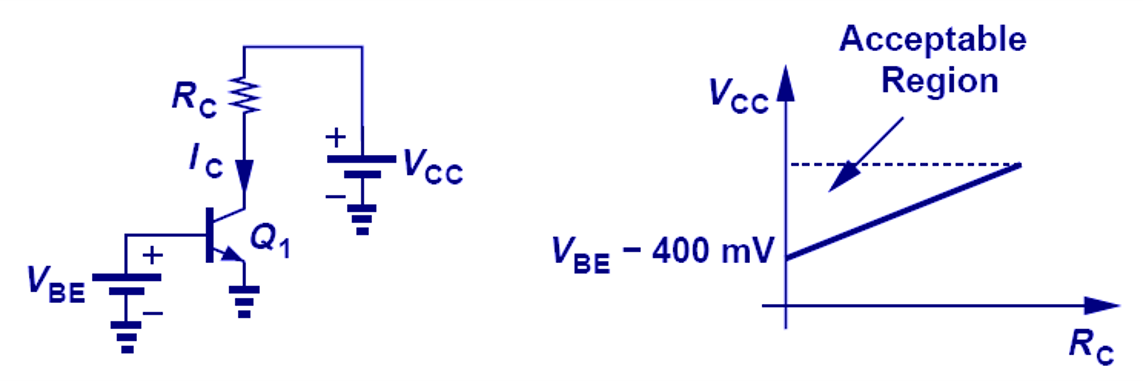
\includegraphics[width=0.7\textwidth]{figures/saturacion_debil.png}
\end{figure}
%
\[ V_{CC} - I_C R_C \geq V_{B} - 400\ mV \]
    
\end{frame}


\begin{frame}{Ejemplo 4: Punto de operación en saturación débil}

\begin{columns}
\begin{column}{0.6\textwidth}

El transistor del circuito mostrado tiene los siguientes parámetros:
%
\[ I_S = 10^{-14}\ A \]
%
\[ \beta = 100 \]
%
\begin{itemize}
    \item Calcule la máxima tensión de la fuente $V_S$ si el transistor debe operar en la región de saturación débil, con una tensión $V_{BC}$ máxima de $400\ mV$.
    \item Realice este problema utilizando ambos modelos (tensión constante y exponencial).
\end{itemize}

\end{column}
\begin{column}{0.4\textwidth}

\begin{figure}
    \centering
    \begin{circuitikz}
        \draw (0,0) node[npn](Q1){$Q_1$};
        \draw (-2,0) to[R] (Q1.base);
        \draw (-1.4,0.8) node[above]{$R_B$};
        \draw (-1.4,0.3) node[above]{$47\ k\Omega$};
        \draw (-2.5,0) -- (-2,0);
        \draw (-2.5,0) to [V] (-2.5,-2);
        \draw (-3,-0.75) node[left]{$V_S$};
        \draw (-3,-1.25) node[left]{$?$};
        \draw (-2.5,-2) node [ground] {};
        \draw (Q1.emitter) -- (0,-2);
        \draw (0,-2) node [ground] {};
        \draw (0,3) to[R] (Q1.collector);
        \draw (0.25,2) node[right]{$R_C$};
        \draw (0.25,1.5) node[right]{$220\ \Omega$};
        \draw (0,3) node[vcc]{$3.3\ V$};
    \end{circuitikz}
\end{figure}

\end{column}
\end{columns}

\end{frame}


\begin{frame}{Solución 4: Punto de operación en saturación débil (V constante)}

\begin{columns}
\begin{column}{0.6\textwidth}

\end{column}
\begin{column}{0.4\textwidth}

\begin{figure}
    \centering
    \begin{circuitikz}
        \draw (0,0) node[npn](Q1){$Q_1$};
        \draw (-2,0) to[R] (Q1.base);
        \draw (-1.4,0.8) node[above]{$R_B$};
        \draw (-1.4,0.3) node[above]{$47\ k\Omega$};
        \draw (-2.5,0) -- (-2,0);
        \draw (-2.5,0) to [V] (-2.5,-2);
        \draw (-3,-0.75) node[left]{$V_S$};
        \draw (-3,-1.25) node[left]{$?$};
        \draw (-2.5,-2) node [ground] {};
        \draw (Q1.emitter) -- (0,-2);
        \draw (0,-2) node [ground] {};
        \draw (0,3) to[R] (Q1.collector);
        \draw (0.25,2) node[right]{$R_C$};
        \draw (0.25,1.5) node[right]{$220\ \Omega$};
        \draw (0,3) node[vcc]{$3.3\ V$};
    \end{circuitikz}
\end{figure}

\end{column}
\end{columns}

\end{frame}



\begin{frame}{Solución 4: Punto de operación en saturación débil (V constante)}

\begin{columns}
\begin{column}{0.6\textwidth}

\end{column}
\begin{column}{0.4\textwidth}

\begin{figure}
    \centering
    \begin{circuitikz}
        \draw (0,0) node[npn](Q1){$Q_1$};
        \draw (-2,0) to[R] (Q1.base);
        \draw (-1.4,0.8) node[above]{$R_B$};
        \draw (-1.4,0.3) node[above]{$47\ k\Omega$};
        \draw (-2.5,0) -- (-2,0);
        \draw (-2.5,0) to [V] (-2.5,-2);
        \draw (-3,-0.75) node[left]{$V_S$};
        \draw (-3,-1.25) node[left]{$?$};
        \draw (-2.5,-2) node [ground] {};
        \draw (Q1.emitter) -- (0,-2);
        \draw (0,-2) node [ground] {};
        \draw (0,3) to[R] (Q1.collector);
        \draw (0.25,2) node[right]{$R_C$};
        \draw (0.25,1.5) node[right]{$220\ \Omega$};
        \draw (0,3) node[vcc]{$3.3\ V$};
    \end{circuitikz}
\end{figure}

\end{column}
\end{columns}

\end{frame}


\begin{frame}{Solución 4: Punto de operación en saturación débil (exponencial)}

\begin{columns}
\begin{column}{0.6\textwidth}

\end{column}
\begin{column}{0.4\textwidth}

\begin{figure}
    \centering
    \begin{circuitikz}
        \draw (0,0) node[npn](Q1){$Q_1$};
        \draw (-2,0) to[R] (Q1.base);
        \draw (-1.4,0.8) node[above]{$R_B$};
        \draw (-1.4,0.3) node[above]{$47\ k\Omega$};
        \draw (-2.5,0) -- (-2,0);
        \draw (-2.5,0) to [V] (-2.5,-2);
        \draw (-3,-0.75) node[left]{$V_S$};
        \draw (-3,-1.25) node[left]{$?$};
        \draw (-2.5,-2) node [ground] {};
        \draw (Q1.emitter) -- (0,-2);
        \draw (0,-2) node [ground] {};
        \draw (0,3) to[R] (Q1.collector);
        \draw (0.25,2) node[right]{$R_C$};
        \draw (0.25,1.5) node[right]{$220\ \Omega$};
        \draw (0,3) node[vcc]{$3.3\ V$};
    \end{circuitikz}
\end{figure}

\end{column}
\end{columns}

\end{frame}


\begin{frame}{Solución 4: Punto de operación en saturación débil (exponencial)}

\begin{columns}
\begin{column}{0.6\textwidth}

\end{column}
\begin{column}{0.4\textwidth}

\begin{figure}
    \centering
    \begin{circuitikz}
        \draw (0,0) node[npn](Q1){$Q_1$};
        \draw (-2,0) to[R] (Q1.base);
        \draw (-1.4,0.8) node[above]{$R_B$};
        \draw (-1.4,0.3) node[above]{$47\ k\Omega$};
        \draw (-2.5,0) -- (-2,0);
        \draw (-2.5,0) to [V] (-2.5,-2);
        \draw (-3,-0.75) node[left]{$V_S$};
        \draw (-3,-1.25) node[left]{$?$};
        \draw (-2.5,-2) node [ground] {};
        \draw (Q1.emitter) -- (0,-2);
        \draw (0,-2) node [ground] {};
        \draw (0,3) to[R] (Q1.collector);
        \draw (0.25,2) node[right]{$R_C$};
        \draw (0.25,1.5) node[right]{$220\ \Omega$};
        \draw (0,3) node[vcc]{$3.3\ V$};
    \end{circuitikz}
\end{figure}

\end{column}
\end{columns}

\end{frame}


\section{Referencias}
\begin{frame}{Lecturas recomendadas}

\begin{itemize}
    \item Razavi, B. (2013). Fundamentals of Microelectronics, 2nd edition. Chapter 4: Physics of Bipolar Transistors, pp. 133-137, Wiley, Los Angeles, California.
\end{itemize}
    
\end{frame}

\end{document}
